% This file was created with tikzplotlib v0.10.1.
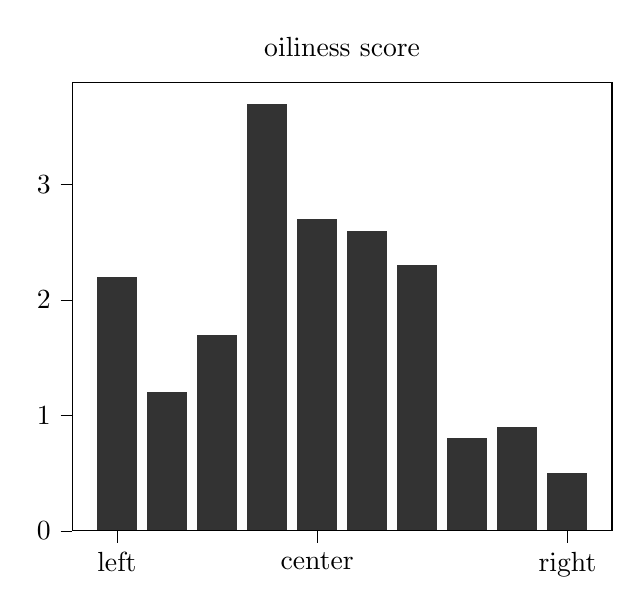
\begin{tikzpicture}

\definecolor{darkgray176}{RGB}{176,176,176}

\begin{axis}[
tick align=outside,
tick pos=left,
title={oiliness score},
x grid style={darkgray176},
xmin=-0.89, xmax=9.89,
xtick style={color=black},
xtick={0,4,9},
xticklabels={left,center,right},
y grid style={darkgray176},
ymin=0, ymax=3.885,
ytick style={color=black}
]
\draw[draw=none,fill=black,fill opacity=0.8] (axis cs:-0.4,0) rectangle (axis cs:0.4,2.2);
\draw[draw=none,fill=black,fill opacity=0.8] (axis cs:0.6,0) rectangle (axis cs:1.4,1.2);
\draw[draw=none,fill=black,fill opacity=0.8] (axis cs:1.6,0) rectangle (axis cs:2.4,1.7);
\draw[draw=none,fill=black,fill opacity=0.8] (axis cs:2.6,0) rectangle (axis cs:3.4,3.7);
\draw[draw=none,fill=black,fill opacity=0.8] (axis cs:3.6,0) rectangle (axis cs:4.4,2.7);
\draw[draw=none,fill=black,fill opacity=0.8] (axis cs:4.6,0) rectangle (axis cs:5.4,2.6);
\draw[draw=none,fill=black,fill opacity=0.8] (axis cs:5.6,0) rectangle (axis cs:6.4,2.3);
\draw[draw=none,fill=black,fill opacity=0.8] (axis cs:6.6,0) rectangle (axis cs:7.4,0.8);
\draw[draw=none,fill=black,fill opacity=0.8] (axis cs:7.6,0) rectangle (axis cs:8.4,0.9);
\draw[draw=none,fill=black,fill opacity=0.8] (axis cs:8.6,0) rectangle (axis cs:9.4,0.5);
\end{axis}

\end{tikzpicture}
